% =============== No Touchy =================== %
\documentclass[11pt, conference, onecolumn]{IEEEtran}

\usepackage{cite}
\usepackage{amsmath,amssymb,amsfonts}
\usepackage{algorithmic}
\usepackage{graphicx}
\usepackage{textcomp}
\usepackage{xcolor}
\usepackage{caption}
\usepackage{subcaption}

\def\BibTeX{{\rm B\kern-.05em{\sc i\kern-.025em b}\kern-.08em
    T\kern-.1667em\lower.7ex\hbox{E}\kern-.125emX}}
\begin{document}

\title{A Portable Tensor Processing Unit\\
}

\author{\IEEEauthorblockN{Wesly Tonks}
\IEEEauthorblockA{\textit{UC Davis}\\
Davis, United States \\
watonks@ucdavis.edu}
\and
\IEEEauthorblockN{Cameron Shinn}
\IEEEauthorblockA{\textit{UC Davis}\\
Davis, United States \\
ctshinn@ucdavis.edu}
\and
\IEEEauthorblockN{Alan Qin}
\IEEEauthorblockA{\textit{UC Davis}\\
Davis, United States \\
aqin@ucdavis.edu}
\and
\IEEEauthorblockN{Skye Develasco}
\IEEEauthorblockA{\textit{UC Davis}\\
Davis, United States \\
sdevelasco@ucdavis.edu}
}

\maketitle

% ============ End No Touchy ==================%

\begin{abstract}
    Trends in computing have led to a proliferation of neural Network applications.
    Unfortunately, todays general purpose processors are not well suited for the class of
    computations these applications require, creating demand for a new class of processors
    : Tensor Processing Units (TPU). These hardware accelerators are designed with neural
    networks in mind, and allow host CPUs to offload computationally expensive
    tensor operations to them. We implement our own, low-power, scalable TPU intended for
    embedded and mobile applications, and evaluate its performance using a simulated
    fully connected neural Network layer.
\end{abstract}

\begin{IEEEkeywords}
Neural Networks, Machine Learning, TPU, Hardware Acceleration
\end{IEEEkeywords}

\section{Introduction}
    % Big Picture
    % Motivation
    % Problem Definition
    % Objective
    With the diminishing of Moore's Law and the exponential increase in data, computing
    needs are out-pacing computing capabilities in general purpose processors in both
    client and server applications. Today's solution is the design of specialized hardware
    co-processors, which specialize in one or a few tasks. These hardware accelerators
    perform complex computations much faster (on the order of 10 - 100 times faster), and
    with much lower power consumption. With the increasing expense of power in all parts
    of the computing spectrum, it is no wonder that hardware accelerators are becoming
    ubiquitous.

    With the creation of data accelerating at an exponential rate, algorithms to
    extrapolate useful information - namely neural networks, have become
    common, and are found in embedded, mobile, and data center applications. These
    algorithms rely heavily on matrix multiplication and convolution, both of which place
    heavy load on today's general purpose processors, creating the need for a Tensor
    Processing Unit (TPU), first commercialized by Google for data center use.

    Note that neural networks have two phases: training and predicting. Both phases are
    computationally expensive, and the topic of cutting edge research. Here, we focus
    on predicting, as much of the neural networks life will be spent making predications,
    rather than training.

    Current TPUs aim to implement the aforementioned matrix multiplication and
    convolution, along with common activation functions used in todays neural networks.
    This is typically done via a highly pipelined data path known as a systolic array,
    which can complete an $N x N$ matrix multiplication in just $2N$ cycles. As with most
    hardware accelerators, TPUs must communicate large amounts of data between itself and
    the host, introducing undesired overhead. TPUs also have large on chip memory
    bandwidth, as the systolic array requires large input and output bandwidth for sustained
    computation.

    The TPU was first introduced by Google in 2013, who was presented with a massive
    amount of compute as their customers began using speech-to-text more often. Over the
    course of 15 months, Google designed and fabricated their fist generation TPU, and
    was able to realize fantastic performance improvements in neural network inference,
    and now uses their TPU as an add in card in their own data centers.

    We present a scaled down, low-power TPU implementation providing performance gains for
    embedded and mobile neural network applications. We aim to increase performance of
    fully connected layers in an application running on an ARM A9 processor. The TPU is
    memory mapped, and communication between the two devices is done via an Avalon bus on
    an Altera DE-1 development kit. The TPU implements a fully pipelined 16 x 16 systolic
    array at a max clock speed of 115 MHz, yielding a noticeable speedup in
    fully connected neural network layers, when compared to the ARM A9 only.

    This implementation allows useful neural Network applications such as image processing,
    object detection, speech-to-text, and more to be run in power and performance limited
    devices such as smart phones and embedded systems. The design is also scalable,
    allowing for a range of hardware configurations per application.
\section{Background}

\subsection{Neural Networks}
    % General description of neural networks here.
    With the advent of big data applications becoming increasingly common, machine learning
    has proved to be the future of complex algorithms. Deep neural networks, a subspace of
    machine learning, are an attempt to reverse engineer the human brain and make computers
    learn and behave like humans. Deep neural networks need to first undergo “training”
    repeatedly with vast amounts of sample data, and self adjusted “synapses”
    (i.e. learning) based on expected results. If given a complete dataset, it is typical
    to use 20\% of the data to train the network, and 80\% to test it. Once a neural
    network has been fully trained, it can then be applied and performs  “inference” on
    whatever it is given. This implies that a domain specific architecture should take
    advantage of the fact that weights will always remain the same, as will be shown later.

    Neural networks are essentially just a series of simple functions applied independently
    to each part of an input. This allows matrices to be used, as matrix operations apply
    the same operation to each piece of the inputs. The downside is that common matrix
    operations such as multiplication and convolution are exceedingly complex, meaning
    general purpose processors (and even GPUs) have low roofline performance for
    neural network inference. Typical neural Network layers implement matrix convolution,
    matrix multiplication, pooling, and an activation function, which is usually ReLU or
    tanh.

    While general purpose processors and graphics processors are certainly capable of
    performing these kinds of operations, they are not specially suited for it.
    Additionally, performance gains due to Moore's law will not provide adequate
    performance increases to meet computing demands put forth by the proliferation of
    neural networks, which are now used in smartphones, data centers, and even cars.

\subsection{Tensor Processing Units}
    % Present the need for Tensor Processing Units
    % Talk about Google's implementation
    % Talk about need for portable, low power TPUs
    Since Moore's law and Denard scaling are coming to an end, industry is adopting
    domain specific architectures which promise extremely high price-performance-power for
    a given set of problems. Google's own TPU is a great example, yielding much greater
    throughput and performance per watt than top GPU's and CPU's in neural Network
    Inference. The success of Google's first generation TPU led to faster and more power
    efficient generations which are now used throughout Google's data centers.

    Google's TPU first came about when their researchers proposed a problem - what
    would happen if every Google user used speech-to-text services for just three minutes
    a day? They found that the amount of compute needed would far exceed the capabilities
    of their CPU and GPU driven data centers, and 15 months later produced a fully
    functional TPU.

    Google's TPU consists of a large $256 x 256$ Systolic array which performs fast matrix
    multiplication. THe systolic array is a 2-dimensional array of processing elements
    (PE's) which are relatively simple execution units. At minimum, they contain a
    registers, a multiply accumulate module, and some control logic. Each PE receives a
    sum, weight, and input matrix element as inputs, and multiplies the input matrix
    element by the weight, then adds that to the sum. The sum is then passed downwards
    to the next PE, while the input matrix element is passed right to another PE. After
    a short transient, Google's Systolic array performs up to $256^2$ multiply-accumulates
    per clock cycle, allowing massive throughput.

    While the large systolic array is capable of massive amounts of compute, it may only
    do so if memories can feed it. Because a set of weights for a given network is usually
    too large to store in on-chip caches, Google uses a DDR3 interface to hold weights,
    put hides memory latency by using Weight FIFO's to prep a set of weights while a
    multiply is taking place. A similar technique is used for the input matrix, which must
    through the 'data set-up' block, as shown below.

    \newpage

    \begin{figure}[htbp]
        \centering
        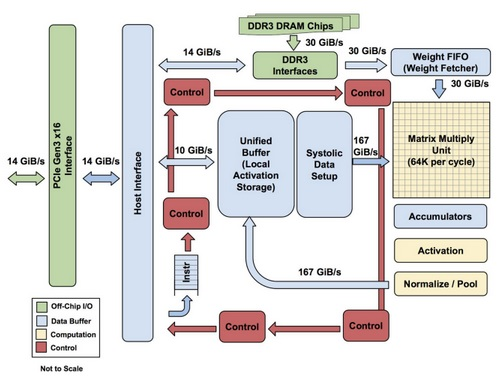
\includegraphics[width=9cm]{../figures/googleArchitecture.jpg}
        \caption{High level view of Google's TPU architecture \cite{b1}}
    \end{figure}

    Google’s original TPU is far more efficient than CPUs and GPUs with 30X to
    80X the energy efficiency (TOPS/Watt), not to mention it’s currently in its third
    generation. The performance of the TPU in a data center environment is unparalleled
    and offers an excellent solution to deep neural network inference in the cloud computing
    space.


\section{Design and Implementation}

    \subsection{System Architecture}
        % Inspiration from Google
        % Include system Architecture figure
        We give credit to Google's TPU as inspiration for our own architecture. Given the
        level of design we are at, resources describing Google's TPU proved very helpful
        in implementing our own.

        A basic overview of our architecture is shown below. Commands and data flow in
        from the host interface, an Avalon AXI bus. These commands are decoded into one of
        the following functions:

        \begin{center}
        \begin{itemize}

            \item{\textit{Write Weight Memory} - Data on the bus is written into a
            specified location in Weight Memory space}

            \item{\textit{Write Input Memory} - Data on the bus is written into a
            specified location in Input Memory space}

            \item{\textit{Fill Weight FIFO's} - A set of weights is read from weight
            memory into the weight FIFO's}

            \item{\textit{Drain Weight FIFO's} - The set of weights currently held in
            the weight FIFOs is loaded into the systolic array}

            \item{\textit{Matrix Multiply} - A set of inputs is piped into the systolic
            array and multiplied with the set of weights currently held in the array.}

            \item{\textit{Read Output Memory} - A specified word from memory is read to
            the host.}
        \end{itemize}
        \end{center}

        \newpage

        \begin{figure}[htbp]
            \centering
            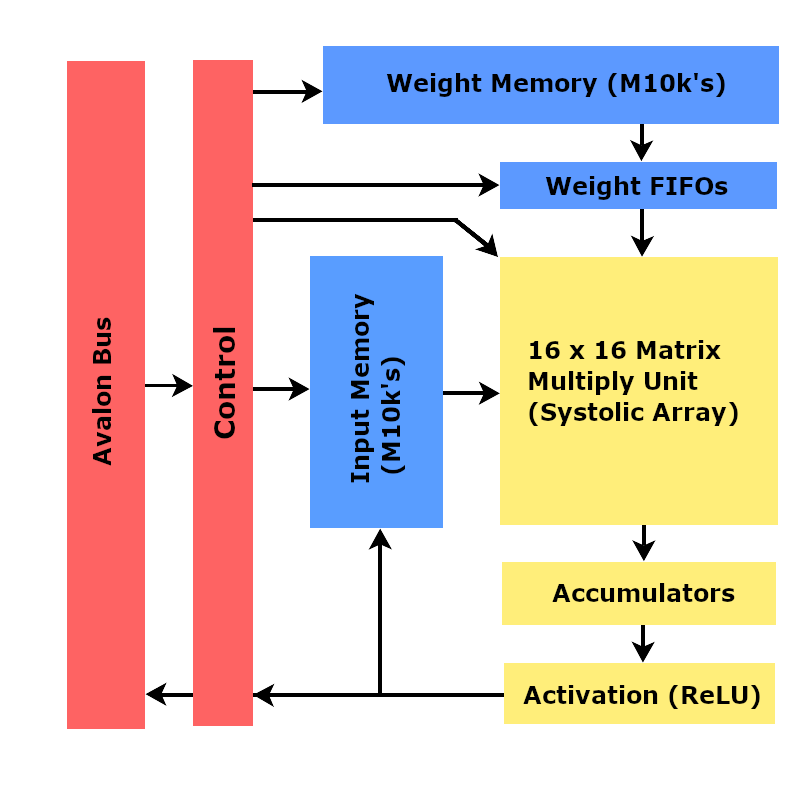
\includegraphics[width=9cm]{../figures/sysArchitecture.png}
            \caption{High level view of system Architecture}
        \end{figure}

    \subsection{Systolic Array}
        % Overview of systolic array
        % Include overview of PE
        % How memory is able to feed the Systolic Array
        Our TPU features a weight stationary systolic array, meaning a set of weights may
        be loaded in once but used for many operations. The array is fully pipelined,
        performing a 16 x 16 matrix multiply in just 32 cycles. It is composed of many
        processing elements (PEs), which contain a small amount of memory and control
        logic, and a single multiply accumulate data path.

        A complete Matrix Multiply starts at the top left corner of the Systolic array,
        and is piped diagonally downward. In the first cycle of a multiply, input memory
        supplies data for only the top left PE. After one cycle, the first PE
        activates its neighbors below and to the right, creating the diagonally downward
        piping.

        Each PE holds one element of the input matrix in any given cycle, and passes that
        element to its right neighbor every cycle. The multiply accumulate result is
        passed downward to the neighbor below every cycle. Each PE then multiplies its
        input element with the weight element stored in it, then adds that value to the
        sum being supplied from its above neighbor. Note that memory interfaces only exist
        at the edges of the systolic array.

        Multiplication results appear at the bottom of the systolic array 16 cycles after
        a multiplication is started, and continue flowing out for 16 cycles. The flow of
        data is illustrated below, showing a scaled down version of our systolic array.

    \subsection{Control}
        The control logic was where we spent the most time debugging, and is what takes
        up most of the ALM's used in the final implementation. We use a single main
        control module which interfaces directly with the bus, decodes signals, then
        drives appropriate control bits in smaller control modules. We have control for
        reading input and weight memories, in which a counter is used to facilitate the
        loading of one entire matrix in 16 clock cycles.

        An output memory control module reads signals from the input memory control, and
        will begin storing outputs from the systolic array into the output memory module.
        For both reading input and weight memory as well as writing output memory, the
        user provides a base address in which the first row of a matrix will be stored,
        and control iterates sequentially through the next 15 addresses until an entire
        matrix has been stored.

        FIFO control logic facilitates the loading of weights into FIFO's above the
        systolic array. It works in tandem with the weight memory control, driving FIFO
        signals as the weight memory control provides data. Note that all control
        modules receive their inputs from the bus control module, which can be considered
        the master controller in the TPU.

    \subsection{Software}
        % Original Goal
        % Drawbacks of hardware
        % Final benchmark
    To demonstrate the capabilities of our TPU, the plan was to train a convolutional
    neural network to benchmark on the TPU. Due to time constraints and technical
    difficulties, this did not happen, but throughout the process we developed a strong
    idea of how we can train a neural network and perform inference on the TPU. The
    convolutional neural network we developed is designed to perform classification of
    diagnoses on chest x-rays. The network takes a grayscale chest x-ray image as an
    input, and outputs any number of 15 classifications, including no diagnosis at all. To
    implement the CNN, we used TinyDNN[7], a simple deep neural network library. The
    choice behind selecting TinyDNN was to have a simple and easy to use library that
    wouldn’t be overwhelming and could be quickly learned under the time constraints for
    this project.

    The network architecture is based on the classic LeNet-5 CNN architecture. Our
    input images are 128 x 128 as opposed to 32 x 32 to preserve the graphical fidelity of
    the chest x-rays, because there is much more detail compared to the 32 x 32 MNIST
    dataset (handwritten digits) that is typically demonstrated on the LeNet architecture.
    Since the input image sizes are larger than LeNet’s input, there are a few adaptations
    that have been made to accommodate this input size: larger convolution kernels
    (5 x 5 up to 9 x 9 on some layers) to break down the size of the layers more; larger
    average pooling grid sizes to cut the results of each layer farther down
    (3 x 3 instead of 2 x 2); removing the feature map in the third layer since it was not
    adaptable to our network architecture. These changes allow us to (presumably) preserve
    the functionality of the LeNet-5 architecture while adapting it to larger inputs.

    To train the neural network, we used the National Institutes of Health Chest X-ray
    Dataset[6] containing over 112,000 chest x-rays from more than 30,000 unique patients.
    Each image had one or more of the 15 classifications discussed earlier (note that if
    the classification is no diagnosis there cannot be any other classification). To groom
    the images for processing we wrote a Python script to resize all of the images to
    128 x 128 and store the 8-bit grayscale pixel values in hexadecimal format in a CSV
    file. Managing and parsing this CSV file became somewhat tedious due to its size, so
    we later moved to using the OpenCV library to do this processing within the training
    code to be stored in a vector at runtime. When performing training, 90\% of the data
    is used for training and 10\% is saved for accuracy analysis at the end.

    The training results are indeterminate. We encountered an issue with the training
    where the network would converge to an approximation that provided the same output for
    any given input image (all output nodes would have the same value). Lightly examining
    some example inputs revealed that the result of each convolutional kernel was
    stripping away the features of the image and the layer values would converge to the
    same value. By the third layer, nearly all of the node values would be the same for a
    given convolution, and by the fourth layer they were all the same. Some things we
    intended to look into were the validity of our architecture and verifying that our
    training data was being interpreted correctly (perhaps some issues with image
    conversion, or some mix-ups between signed and unsigned values). Unfortunately we
    couldn’t afford to allocate much time to this issue as it was too late in the project
    timeline. To compromise, we just decided we would benchmark a set of random weight
    values instead.

    \begin{figure}[htbp]
        \centering
        \includegraphics[width=0.8\linewidth]{../figures/nn.png}
        \caption{Our network architecture. Based off of the LeNet-5 architecture.}
    \end{figure}


\section{Results}
    % Discuss Quality of implementation
    % Observed Speedup
    \subsection{Final Implementation}
        The final implementation of our TPU is quite simple. It is driven by the 16 x 16
        systolic array described above, which supports pipelined matrix multiplies. The
        systolic array is fed by a robust memory system, having a 256 deep 8-bit word
        memory for each row and column (for inputs and weights), as well as another 256
        deep 8-bit word memory for each column for outputs.

        The final FPGA fabric usage is lower than expected, using only 112,000 memory bits,
        and less than 10\% of the interconnect, and around 25\% of the ALM's. We are
        nearly maxed out in terms of DSP block usage, using 64 out of the provided 81 for
        the systolic array. Note that the low usage of interconnect and ALM's allows room
        for future optimizations, described below.

        \begin{figure}[htbp]
            \centering
            \includegraphics[width=0.4\linewidth]{../figures/chipPlanner2.png}
            \caption{Quartus Chip Planner tool showing overall FPGA usage. Note the
                long stripes spreading the design out; these are the DSP blocks.}
        \end{figure}

    \subsection{Benchmarking}
        The benchmarking suite designed for the TPU ran $2^{16}$ 16 x 16 matrix multiplies,
        once using only the ARM A9 processor, and once using the ARM A9 in tandem with
        our TPU. This test bench is meant to model fully connected layers in neural
        networks. We run three cases for TPU usage; one worst case scenario, in which every
        multiplication must have inputs, outputs, and weights written/read over the bus,
        one average case scenario, in which we re-use weights, and one throughput only
        scenario, in which we do no bus transfers in order to test throughput of our
        systolic array. The final scenario also allows us to benchmark the performance of
        bus. Note that all three benchmarks are run with full compiler optimizations.

        In the worst-case bus usage scenario, our TPU is able to outperform the ARM A9
        with a 1.6 times speedup. This is great, as even in a worst case scenario, our
        simple TPU is able to outperform a relatively strong mobile processor. This worst
        scenario is defined by having each multiply require that inputs, weights, and
        outputs be written/read before/after every multiply. While this would not be a
        common use case for our TPU, we feel it is important to demonstrate a worst case
        performance metric for our design.

        In the more extreme no bus usage scenario, we can see the extremely high throughput
        achieved by the Systolic Array. In this test, our TPU achieves a throughput of
        $1.39$ Gops/s, nearly ten times that of the ARM A9! We infer that this
        immense throughput is what makes up for the long latency of bus transactions
        present in the other two benchmarks, and infer that using a more robust
        host-TPU interconnect would greatly benefit our design.

        The average case bus usage scenario, in which only some multiplies must do a
        full input, weight, and output write/read, we see higher performance gains over
        the ARM A9, up to about a doubling in performance. This use case attempts to model
        an application which only processes using a single set of weights at a time, such
        that weights need not be sent to the TPU for every multiply, as would be common
        in neural network applications.

        \begin{figure}[htbp]
            \centering
            \includegraphics[width=0.8\linewidth]{../figures/runtime.png}
            \caption{Average runtime of a series of matrix multiplications under several
                     use cases}
        \end{figure}

        \newpage

        \begin{figure}[htbp]
            \centering
            \includegraphics[width=0.8\linewidth]{../figures/throughput.png}
            \caption{Average throughput of matrix multiplications under several use cases}
        \end{figure}

        As a note, this testbench assumes each instruction sent to the TPU must finish
        before the next instruction may be issued. This allows for simple software-side
        instructions which issue the command and data, then idle until the corresponding
        done signal is received. While this implementation simplifies the software usage,
        it does not allow the TPU to utilize its instruction level parallelism. Since our
        Systolic array is fully pipelined, multiplies may be issued on every TPU clock
        cycle. Additionally, input, output, and weight memory may be written/read while
        the TPU is performing a multiply, allowing us to hide the latency of bus
        interaction.

        As another note, the ARM A9 processor was running as a serial program. A
        common optimization would be to use pthreads or OpemMP to spawn separate threads
        which can run matrix multiplications in parallel, taking advantage of the A9's
        second core. This would likely place the A9 on par with the average and worst case
        performance metrics produced by our TPU.

\section{Future Work}
    % There is plenty of room for improvement of the TPU we have implemented...
    Although this first TPU iteration is able to successfully accelerate a fully connected
    deep neural network, there are some hardware limits and optimizations that should be
    discussed. The two most discernible improvements are pipelined PEs and a more capable
    Host-TPU bus. There are also software side improvements to be made, which would allow
    full hardware utilization and easy implementation of applications on the TPU.

    With the system clock frequency being limited to 115 MHz, the critical path is the
    arithmetic in the PEs of the systolic array. In the current design, each PE is its own
    pipestage, meaning it performs an 8-bit multiply and a 16-bit addition all in one
    clock cycle. If the process elements were registered between the multiply and
    accumulate, then there would be a significant speedup in the maximum operable
    frequency. This optimization would increase the latency of a multiply, but increase the throughput, as a single multiply would now take 64 cycles instead of 32. Note that a
    significant amount of our control modules would have to change as well.

    In the benchmarks for the current design, it is clear that bus transfers dominate our
    execution time. A full set of bus transactions (input write, weight write, output
    read) takes roughly twice as much execution time as a matrix multiplication. As per
    Amdahl’s law, this design would benefit more from improvements in bus transfer time.
    The current implementation of the Avalon bus does not take full advantage of our
    memory throughput capabilities; it has half the throughput of the memory, so this
    design would benefit from up 2x bus throughput. This could be done using the DMA
    burst transfer feature of the Avalon bus.

    One last thing is that our group didn’t have a change to fully implement the
    instruction set, but had nearly all the pieces there. Having a working instruction set
    would make the TPU a lot easier to control via software. The instruction function
    calls would handle the bus operations automatically, and would simply have the
    relevant arguments with their own fields in each instruction. Lack of time is why this
    plan didn’t come to fruition, so it would be one of the first things to check off of
    the list.

    In addition to the potential improvements to the current design, there is also extra
    hardware functionality that could be added to make the TPU more robust. In the future
    these are features that will be looked into in future iterations of this TPU. These
    features we’d like to explore are a separate datapath for convolution, multiple weight
    registers to the PEs and a better programming interface.

    In our TPU, there isn’t any hardware specific to performing convolution, and in
    Google’s we believe there is a very minimal amount of hardware support as well.
    It has already addressed how convolution can be done within the systolic array, but
    the matter of fact is that it is largely inefficient unless processing multiple
    kernels simultaneously, which may not always be a luxury that is available. This is
    due to the fact that a kernel must be contained in a column of the weight matrix, so
    performance can only be maximized by filling up every column with a different kernel.
    Instead, having a separate datapath for an efficient convolution module to issue
    convolution instructions to would increase the overall throughput of tensor processing
    by keeping the systolic array freed up from inefficient computations.

    One other issue with the current design is that there is no reliable way to quickly
    switch between weights. The only way weights can be changed is by emptying the weight
    FIFO to overwrite the weights in the systolic array. This is a very slow process and
    can result in a lot of wasted time if the TPU is going back and forth between a few
    sets of weights. This issue is similar to thrashing of data in caches; reusing the
    same few pieces of data, but having to pay the cost of loading them back in every time
    because there is not enough space to store them all. A good solution to this would be
    to have more weight registers in the PEs of the systolic array and an index control
    signal that indicates which set of weights should be used for a give multiply
    accumulation (note that this control only needs to be driven to the top left element
    of the systolic array like other control signals). For example, an entire 16 layer
    deep neural network could have all of its weights loaded into the systolic array as
    they are needed so that there is no concern over the order in which a batch of input
    data is processed. The weights could be easily switched between in a given clock cycle
    with a simple 4-bit index value.

    One last feature that would make using the TPU much easier would be providing a more
    programmable interface. Right now, the simple TPU instruction set would require a fair
    amount of knowledge about the hardware to achieve maximum performance. As an interface
    it is not very easy to work with. From a programmers point of view, the hardware
    should be abstracted so that a user wouldn’t need to know a thing about it to achieve
    reasonable performance gains in their code. A good addition would be to write drivers
    for our device so that there is a more friendly, higher level user interface that can
    automate the instruction ordering. This could be in the form of a library that can
    process a batch of information at a time, whether it be matrix multiplication or
    tensor processing on a set of inputs.

\begin{thebibliography}{00}
\bibitem{b1} Patterson, D., Jouppi, N. and Young, C. (2017). In Datacenter Performance of A Tensor Processing Unit. 44th International Symposium on Computer Architecture.
\bibitem{b2} Patterson, D., Hennesy, J. (2019). Computer Architecture, A Quantitative Approach. Sixth Edition. Morgan Kaufmann Publishers
\bibitem{b3} Telesens.co (2018) Understanding Matrix Multiplication on a Weight-Stationary Systolic Architecture Web
\bibitem{b4} K. Kiningham, M. Graczyk and A. Ramkumar, "Design and Analysis of a Hardware CNN Accelerator", 2017.
\bibitem{b5} Shaaban, "Systolic Architectures", Portland State University, 2003.
\bibitem{b6} [4]"Random Sample of NIH Chest X-ray Dataset", kaggle.com, 2017. [Online]. Available: https://www.kaggle.com/nih-chest-xrays/sample.
\bibitem{b7} nyanp et. al. "tiny-dnn", (2012 - 2019), GitHub Repository, https://github.com/tiny-dnn/tiny-dnn.
\end{thebibliography}
\end{document}
